\documentclass[12pt, a4]{article}
\usepackage[english]{babel}
\usepackage[utf8x]{inputenc}
\usepackage{fullpage}
\usepackage{listings}
\usepackage{graphicx}
\usepackage{color}

%Syntax highlighting
\definecolor{blue-violet}{rgb}{0.54, 0.17, 0.89}
\definecolor{ao}{rgb}{0.0, 0.5, 0.0}
\definecolor{amaranth}{rgb}{0.9, 0.17, 0.31}
\definecolor{ballblue}{rgb}{0.13, 0.67, 0.8}
\definecolor{onyx}{rgb}{0.06, 0.06, 0.06}


\lstset{
  breaklines=true,                 % automatic line breaking only at whitespace
  captionpos=b,                    % sets the caption-position to bottom
  breakatwhitespace=false,
  keepspaces=true,
  numbers=left,
  numbersep=5pt,
  showspaces=false,
  showstringspaces=false,
  showtabs=false,
  tabsize=4,  
  backgroundcolor=\color{white},   % choose the background color
  commentstyle=\color{ao},    % comment style
  keywordstyle=\color{amaranth},    % keyword style
  stringstyle=\color{blue-violet},    % string literal style
  numberstyle=\tiny\color{ballblue},	   % number style
  basicstyle=\ttfamily\footnotesize\color{onyx} % size of fonts used for the code
}

%Document Header
\title{\textbf{Department of CSE\\SSN College of Engineering}}
\author{\textbf{Vishakan Subramanian - 18 5001 196 - Semester VI}}
\date{22 January 2021}

\begin{document}
\maketitle
\hrule
\section*{\center{UCS 1602 - Compiler Design}}
\hrule
\bigskip

%Assignment Details
\subsection*{\center{\textbf{Exercise 1: Lexical Analyser Using C}}}
\subsection*{\flushleft{Aim:}}
\begin{flushleft}
To write a program using C to perform the
basic functionalities of a \textbf{Lexical Analyser}.
\end{flushleft}

%Code
\newpage
\subsection*{\flushleft{Code:}}
\begin{flushleft}
\lstinputlisting[language = C, firstline = 1, lastline = 394]{Lex.c}
\end{flushleft}

%Output
\newpage
\subsection*{\flushleft{Output - Valid Case:}}
\begin{figure}[h]
\centering
\caption{Console Output for a Valid Program.}
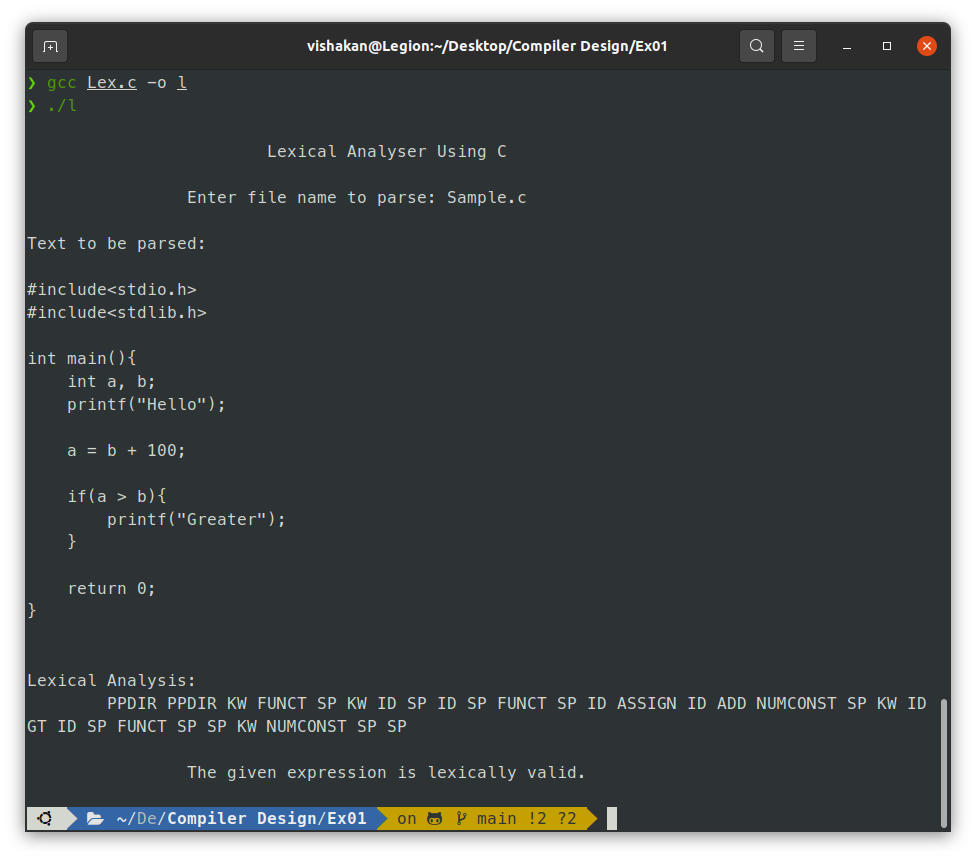
\includegraphics[scale= 0.5]{valid_example.png}
\end{figure}

\newpage
\subsection*{\flushleft{Output - Invalid Case:}}
\begin{figure}[h]
\centering
\caption{Console Output for an Invalid Program.}
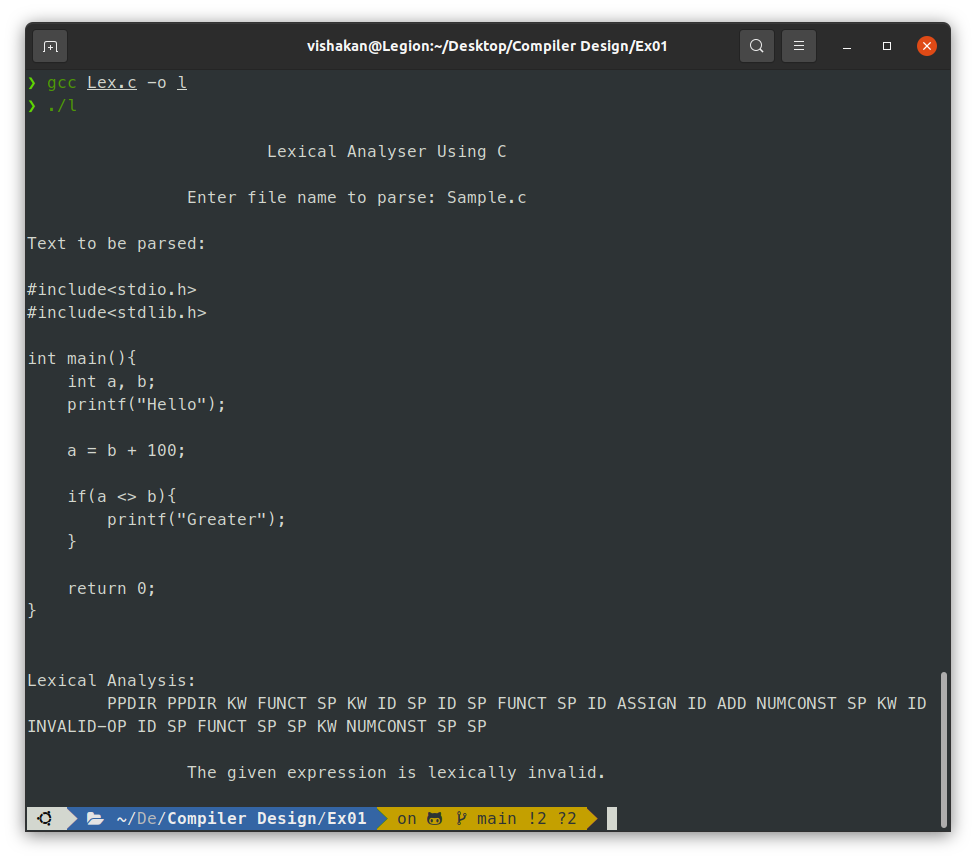
\includegraphics[scale= 0.5]{invalid_example.png}
\end{figure}

%Learning Outcome
\newpage
\subsection*{\flushleft{Learning Outcome:}}
\begin{itemize}

\item From the experiment, I understood how a basic \textbf{Lexical Analyser} works.
\item I was able to formulate ideas on how to implement recognition of specific tokens in programs for identification by the Lexical Analyser. 
\item I was able to implement simple regular expressions in C.
\item I learnt how to parse a program for lexical validity, utilising the concept of \textbf{lexemes}.
\item I was able to visualize the complexity that goes behind the compilation process and the significance of a Lexical Analyser phase in the compilation flow.

\end{itemize}


\end{document}